\documentclass[letterpaper,11pt]{article}
\usepackage[letterpaper,bottom=2.5cm,top=1cm,left=2.5cm]{geometry}
\usepackage[spanish]{babel}
\usepackage[utf8]{inputenc}
\usepackage{hyperref}
\usepackage{graphicx}
\usepackage{csquotes}



\bibliographystyle{apalike}



\title{HOLA JUANCHOOOOOO}
\author{Juan Crespo  \\  \url{jp.crespo.vargas@gmail.com}}

\date{} % si no la pongo se pone automáticamente
  
\begin{document}
\maketitle


\begin{abstract}
  
\end{abstract}
  
\section{Introducción}
\label{sec:intro}
La energía que llega del Sol en forma de luz (fotones) a nuestro planeta permite que se lleve a cabo el proceso de la vida. Esta energía se transmite mediante ondas electromagnética, las cuales dependiendo de la energía que portan tienen distintas interacciones en la materia. 

Afortunadamente el planeta tierra filtra la mayoría de ondas nocivas para el material biológico, permitiendo el paso de las ondas menos energéticas que provengan del sol y del espacio profundo.

Sin embargo las ondas filtradas que ingresan a la atmósfera tienen un rango relativamente amplio de energías que a su vez son filtradas por el aire hasta llegar a la superficie terrestre. En el caso de lugares con mayor altura sobre el nivel del mar, la llegada de radiación solar es más intensa. Esta radiación solar produce efectos adversos sobre el tejido epidérmico (la piel), que pueden derivar en enfermedades como el melanoma (una tipo de cáncer). El efecto de la radiación solar sobre la piel como las razones del porque sucede esta enfermedad en la piel (cáncer de piel) son bien conocidas y están relacionadas con la energía de la luz solar en el rango ultravioleta. Existen laboratorios especializados en el estudio de la física de la atmósfera como por ejemplo, el Laboratorio de Ozono y Radiación Ultravioleta (LORUV) dependiente del Instituto de Investigaciones Físicas de la Universidad Mayor de San Andrés, que estudian y monitorizan los niveles de radiación solar y brindan sus recomendaciones para el cuidado de la salud. 

Durante el año 2020 se desencadeno una Pandemia a escala Global a raíz de la transmisión aérea de una cepa de coronavirus no conocida, el SARS-CoV-2. Entre las múltiples investigaciones a raíz de esta Pandemia se estudió la capacidad de esterilización de la luz solar \cite{covidsol} sobre el nuevo coronavírus. Simularon en laboratorio condiciones de luz solar ambiental a nivel del mar en un día claro de verano, reportando que se necesitan solo 6,8 minutos para inactivar el 90\% del virus en una superficie expuesta. En el estudio también se identifica que es el componente ultravioleta (UVA-UVB) de la luz solar quien tiene el efecto esterilizante. 

En el presente estudio se aborda el uso de radiación ultravioleta (UV) artificial para la esterilización eficiente de superficies y ambientes.

\section{Espectro Electromagnético}  

Una onda electromagnética se caracteriza por su frecuencia o su longitud de onda. El producto de ambos es una constante invariante, la velocidad de la luz. Para calcular la energía asociada a una onda electromagnética se utiliza la relación de Planck:
\begin{equation}
E= h * \lambda
\label{plank}
\end{equation}

Siendo $\lambda$ la frecuencia de la onda.

En la figura \ref{espectro} se muestra de manera general el espectro electromagnético. Contiene una comparativa con las distintas frecuencias de una onda electromagnética y los tamaños con los que puede interactuar en la materia. 
El tamaño de un virus es mucho menor al de los protozoos pero al estar compuesta de múltiples moléculas, en la figura \ref{espectro} correspondería a una onda entre el rango ultravioleta.Preferentemente usaremos la longitud de onda para caracterizar la energía asociada a la onda electromagnética. 

Se denomina espectro visible al rango del espectro electromagnético que el ojo humano es capaz de percibir, cada color se puede representar en función de la longitud de onda. El rango visible se encuentra entre los 380  

\begin{figure}[hbt!]
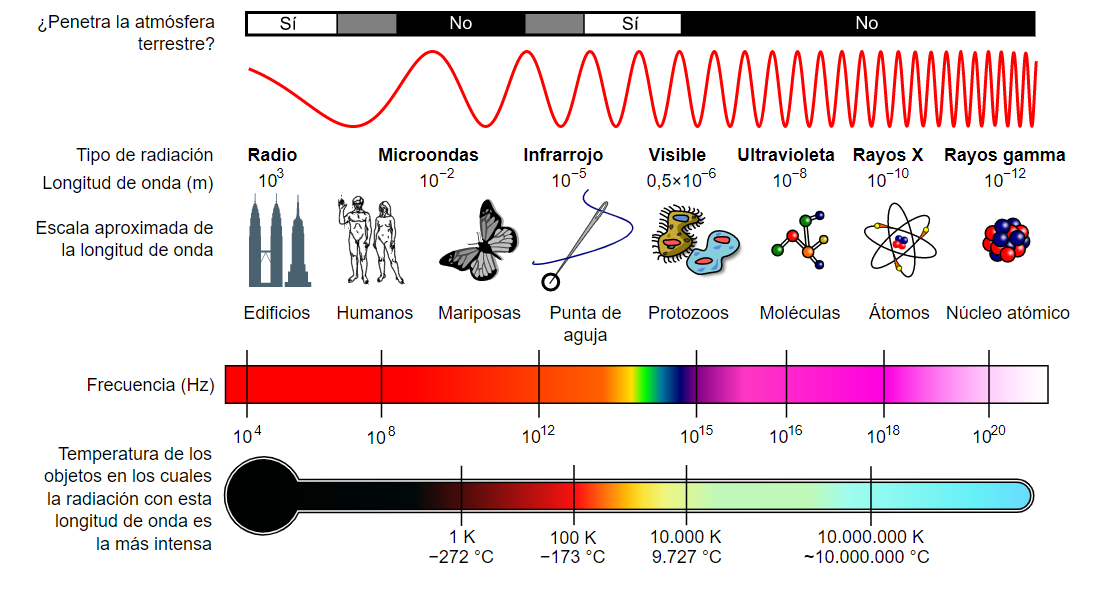
\includegraphics[width=\textwidth,scale=0.3]{espectro.png}
\caption{Espectro Electromagnético}
\label{espectro}
\end{figure}



\bibliography{bibliografia.bib}
\end{document}


